% Created 2021-01-17 Sun 17:33
% Intended LaTeX compiler: pdflatex
\documentclass{beamer}\usepackage{listings}
\usepackage{color}
\usepackage{amsmath}
\usepackage{array}
\usepackage[T1]{fontenc}
\usepackage{natbib}
\lstset{
keywordstyle=\color{blue},
commentstyle=\color{red},stringstyle=\color[rgb]{0,.5,0},
literate={~}{$\sim$}{1},
basicstyle=\ttfamily\small,
columns=fullflexible,
breaklines=true,
breakatwhitespace=false,
numbers=left,
numberstyle=\ttfamily\tiny\color{gray},
stepnumber=1,
numbersep=10pt,
backgroundcolor=\color{white},
tabsize=4,
keepspaces=true,
showspaces=false,
showstringspaces=false,
xleftmargin=.23in,
frame=single,
basewidth={0.5em,0.4em},
}
\usepackage{natbib, dsfont, pgfpages, tikz,amssymb, amsmath,xcolor}
\setbeamertemplate{footline}[frame number]
\beamertemplatenavigationsymbolsempty
\usepackage{appendixnumberbeamer}
\bibliographystyle{abbrvnat}
% New operators and commands
\newcommand{\Z}{\mathbb{Z}}
\newcommand{\Q}{\mathbb{Q}}
\newcommand{\R}{\mathbb{R}}
\newcommand{\N}{\mathbb{N}}
\newcommand{\C}{\mathbb{C}}
\renewcommand{\S}{\mathbb{S}}
\newcommand{\blank}{\makebox[1ex]{\textbf{$\cdot$}}}
\newcommand\independent{\protect\mathpalette{\protect\independenT}{\perp}}
\def\independenT#1#2{\mathrel{\rlap{$#1#2$}\mkern2mu{#1#2}}}
\renewcommand{\phi}{\varphi}
\renewcommand{\epsilon}{\varepsilon}
\newcommand*\diff{\mathop{}\!\mathrm{d}}
\newcommand{\weakly}{\rightsquigarrow}
\newcommand\smallO{
  \mathchoice
    {{\scriptstyle\mathcal{O}}}% \displaystyle
    {{\scriptstyle\mathcal{O}}}% \textstyle
    {{\scriptscriptstyle\mathcal{O}}}% \scriptstyle
    {\scalebox{.6}{$\scriptscriptstyle\mathcal{O}$}}%\scriptscriptstyle
}
\newcommand{\midd}{\; \middle|\;}
\newcommand{\1}{\mathds{1}}
\usepackage{ifthen} %% Empirical process with default argument
% \newcommand{\G}[1][]{%
%    \ifthenelse{ \equal{#1}{} }
%       {\ensuremath{\mathbb{G}_n}}
%       {\ensuremath{\mathbb{G}_{#1}}}
% }
% New version:
\newcommand{\G}[2][n]{
{\ensuremath{\mathbb{G}_{#1}}{\left[#2\right]}}
}
\DeclareMathOperator*{\argmin}{\arg\!\min}

% New operators for consistent notation
\newcommand{\V}{\mathrm{Var}} % variance
\newcommand{\measure}[1]{\mathrm{{#1}}} % measure
% \newcommand{\measure}[1]{\textnormal{\textbf{{#1}}}} % measure
\newcommand{\m}[1]{\measure{#1}} % measure shortcut
\newcommand{\eqd}{\stackrel{d}{=}} % equality in distribution
\newcommand{\arrow}[1]{\xrightarrow{\; {#1} \;}}
\newcommand{\arrowP}{\xrightarrow{\; \m{P} \;}} % convergence in probability
\newcommand{\leb}{\lambda} % the Lebesgue measure
\newcommand{\T}{\top} % transpose
\newcommand{\KL}{\ensuremath{D_{\mathrm{KL}}}}

\usepackage{xargs}
% Make it easy to change counterfactual notation:
\newcommandx{\cf}[4][3={}, 4={}]{
  % \ifthenelse{ \equal{#4}{} }
  % {{#1^{#2}}(#3)}
  {\ifthenelse{ \equal{#3}{} }
    {{#1^{#2}}_{#4}}
    {{#1^{#2}}_{#4}(#3)}}
}

% Easily change notation:
\DeclareMathOperator{\TT}{\Psi} % target parameter
\newcommand{\lp}{\mathcal{L}_{\P}^2} % shortcut for lp2 space
\newcommand{\empmeas}{\hat{\mathbb{P}}_n} % empirical measure
\DeclareMathOperator{\E}{\mathbb{E}} % expectation
\renewcommand{\P}{\m{P}} % probability
\newcommand{\ic}{\mathrm{IF}} % influence curve

\renewcommand*\familydefault{\sfdefault}
\itemsep2pt
\usepackage[utf8]{inputenc}
\usepackage[T1]{fontenc}
\usepackage{graphicx}
\usepackage{grffile}
\usepackage{longtable}
\usepackage{wrapfig}
\usepackage{rotating}
\usepackage[normalem]{ulem}
\usepackage{amsmath}
\usepackage{textcomp}
\usepackage{amssymb}
\usepackage{capt-of}
\usepackage[colorlinks=true]{hyperref}
\usetheme{default}
\author{Anders Munch}
\date{September 30, 2020}
\title{Genes, life-course and heart failure -- intro to PhD project}
\begin{document}

\maketitle
\section{Structure}
\label{sec:org35f3b03}
\begin{frame}[label={sec:orgedeb247}]{Introduction to PhD project}
\begin{itemize}
\item The problem
\item The data
\item Some thoughts/ideas so far
\end{itemize}
\end{frame}

\section{Overall setting}
\label{sec:org3f40a48}
\begin{frame}[label={sec:org0e0a31e}]{People involved}
\begin{itemize}
\item Thomas Gerds and Claus Ekstrøm from here
\item Christian Torp-Pedersen, Professor of Cardiology and Senior Consultant, Gentofte Hospital and University of Copenhagen
\item Charlotte Andersson, MD PhD, Herlev Hospital and Boston Medical Center
\end{itemize}
\end{frame}

\begin{frame}[label={sec:orgc668c64}]{Overall motivation / ``hypothesis''}
\begin{itemize}
\item Better understanding of the causes of HF. In particular a focus on the genetic effects. \pause
\item Heterogeneous disease / syndrome. \pause
\item Better HF sub-diagnoses or disease pattern \(\rightarrow\) identify genetic effects. \pause
\item Use machine learning for this \ldots{}
\end{itemize}
\end{frame}

\begin{frame}[label={sec:org68519aa}]{Data}
\begin{description}
\item[{Coronary arteries examiniation:}] \(\sim 6,000\) individuals + DST data. Weird selection criteria,
non-representative population.
\item[{Blood donors:}] \(\sim 300,000\) individuals in ``computer room''. Very healthy individuals.
\item[{Framingham:}] Participants from a small city. Detailed medical information measured repeatedly
over many years and generations. Genetic data for later generations.
\end{description}
\end{frame}

\section{Clustering of diseases patterns leading to HF}
\label{sec:org8814959}
\begin{frame}[label={sec:org86ad4b4}]{Initial thoughts}
\begin{columns}
\begin{column}{.4\columnwidth}
\begin{block}<2->{\center Cluster disease patterns}
\end{block}

\begin{block}<3->{\center Mediation}
\end{block}

\begin{block}<4->{\center \(\downarrow\)}
\end{block}

\begin{block}<4->{\center Local independence?}
\end{block}
\end{column}

\begin{column}{0.5\columnwidth}
\begin{center}
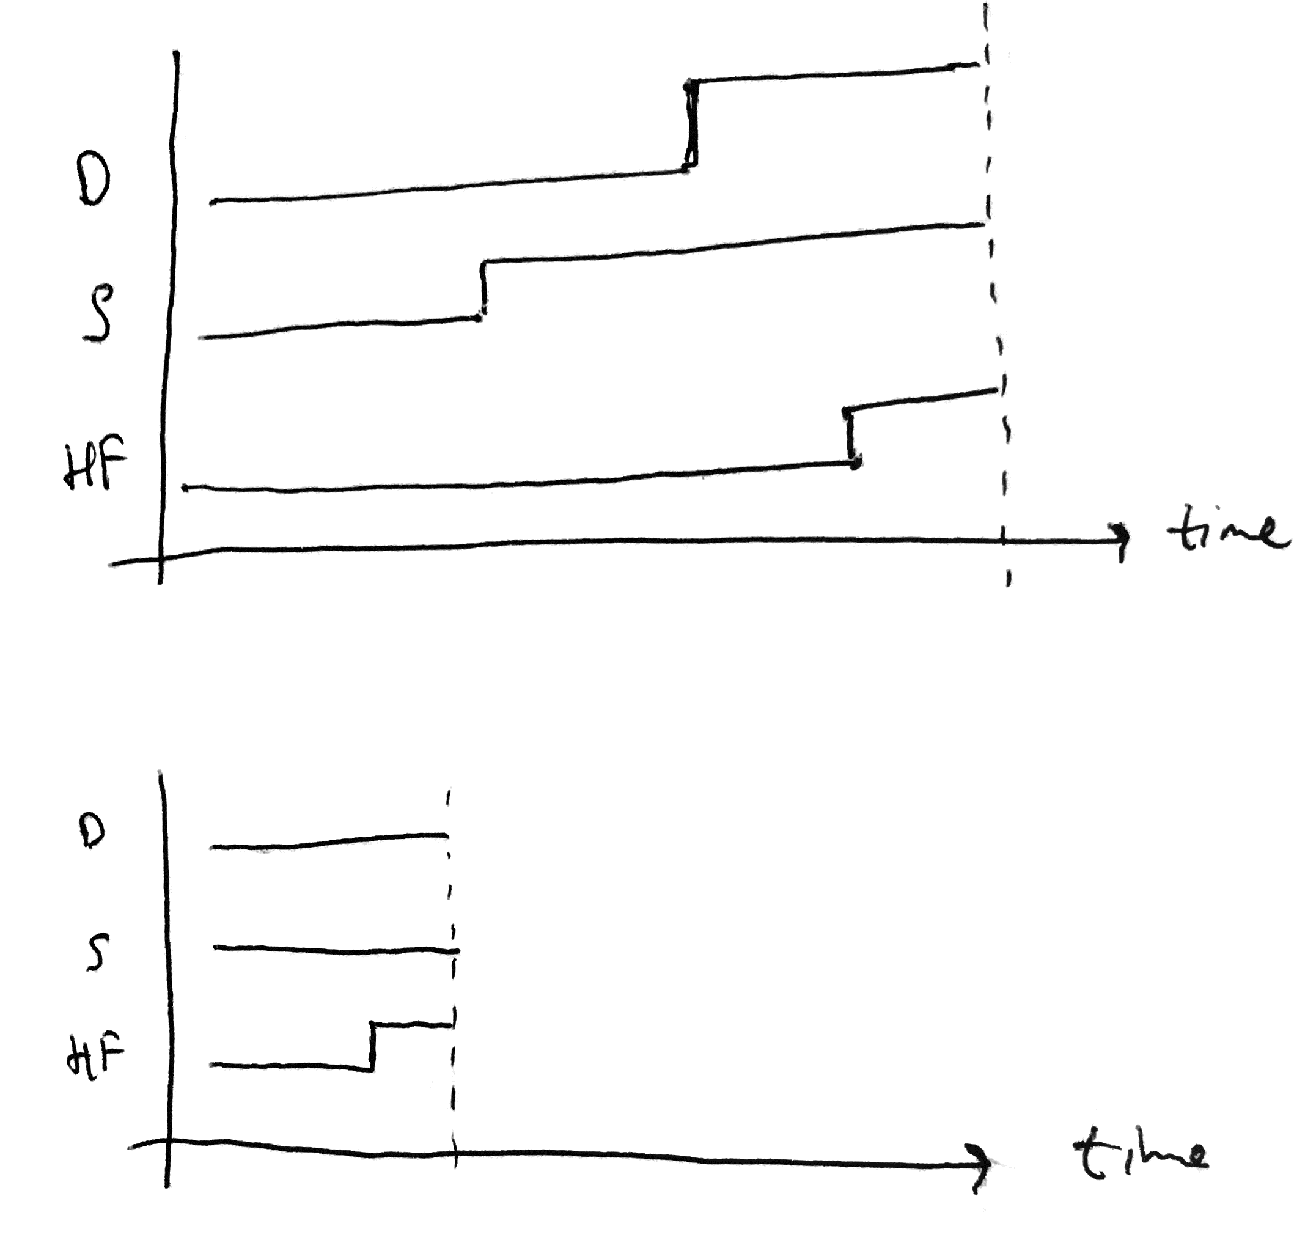
\includegraphics[width=.9\linewidth]{./figs/disease-pattern-drawing.pdf}
\end{center}
\end{column}
\end{columns}
\end{frame}

\section{Setting}
\label{sec:org4bd22e3}
\begin{frame}[label={sec:orgca8c267}]{Formalization of the problem}
\begin{block}{One rough initial formalization}
We observe a multivariate process $ X = (G, D, Y)$,
\begin{equation*}
  Y(t), \quad D(t), \quad G(t) = G, \quad t \in [0, T],
\end{equation*}
where $Y \in \{0, 1\}$ denotes if heart failure has occurred, $D$ denotes status of some disease
(for instance diabetes or not at time $t$), $G$ is constant and contains genetic information, and
$T$ is time of death.
\pause
\end{block}

\begin{block}{Later}
\begin{itemize}
\item much more complicated \(D\)
\item very high-dimensional \(G\)
\end{itemize}

For now, focus on the time dynamic issues so we assume both are one-dimensional.
\end{block}
\end{frame}

\begin{frame}[label={sec:org07792b3}]{Informal questions we might want to ask}
\pause
\begin{itemize}
\item Are there some particular disease patterns for which the genetic disposition is particularly
important for the risk of HF?
\end{itemize}
\pause
\begin{itemize}
\item How does the genetic mechanisms work? Direct influence on the risk of HF or indirect influence
through increased risk of precursors for HF?
\end{itemize}

\pause
\begin{block}{Doubtful illustrations}
\def\shift{3}
\begin{center}
\begin{tikzpicture}
  \node[] (G) at (0,0) {G};
  \node[] (D) at (1,1) {D};
  \node[] (Y) at (2,0) {Y};
  \draw[->] (G) -- (D);
  \draw[->] (G) -- (Y);
  \draw[->] (D) -- (Y);

  \node[] (G) at (0 + \shift,0) {G};
  \node[] (D) at (1 + \shift,1) {D};
  \node[] (Y) at (2 + \shift,0) {Y};
  \draw[->] (G) -- (D);
  \draw[->] (D) -- (Y);

  \node[] (G) at (0 + \shift *2,0) {G};
  \node[] (D) at (1 + \shift *2,1) {D};
  \node[] (Y) at (2 + \shift *2,0) {Y};
  \draw[->] (G) -- (Y);
  \draw[->] (D) -- (Y);
\end{tikzpicture}
\end{center}

What does the above mean when \(D\) and \(Y\) are processes?
\end{block}
\end{frame}

\section{Local independence}
\label{sec:orgcc6af39}
\begin{frame}[label={sec:orga2665f4}]{Local independence}
\pause
\begin{definition}[Informal]
For a multivariate stochastic $X$
\begin{equation*}
  X(t) = (X^1(t), X^2(t), \dots, X^k(t)), \quad t \in [0, T], 
\end{equation*}
with $V:=\{1, \dots, k\}$, we say that for $A, B, C \subset V$, $X^B$ is \textit{locally
  independent} of $X^A$ given $X^C$ if
\begin{equation*}
  X^B(t) \independent X^A([0,t)) \mid X^C([0,t)), \quad \forall t \in [0, T].
\end{equation*}
This is written as $  A \not \rightarrow B \mid C$.

\pause
\end{definition}
\begin{block}<2->{}
"In words, the process $X^B$ is locally independent of $X^A$ given $X^C$ if, for each time point,
the past up until time $t$ of $X^C$ gives us the same \textit{predictable} information about
$\E[X^{\beta}(t) \mid \mathcal{F}_t^{A\cup C}]$ as the past of $X^{A \cup C}$ until time $t$." \citep{mogensen2020markov}
\end{block}
\end{frame}
\begin{frame}[label={sec:org328bd26}]{Local independence -- visualization}
\begin{onlyenv}<+>
\begin{center}
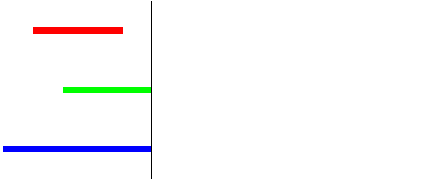
\includegraphics[width=.9\linewidth]{./figs/dyn-sys1.pdf}
\end{center}
\end{onlyenv}

\begin{onlyenv}<+>
\begin{center}
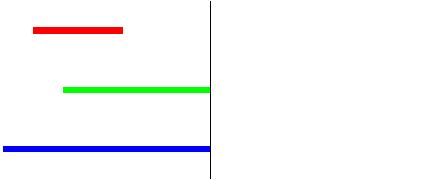
\includegraphics[width=.9\linewidth]{./figs/dyn-sys2.pdf}
\end{center}
\end{onlyenv}

\begin{onlyenv}<+>
\begin{center}
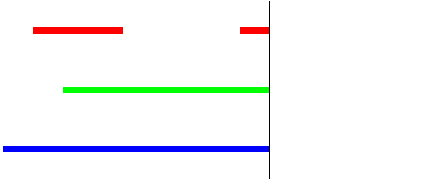
\includegraphics[width=.9\linewidth]{./figs/dyn-sys3.pdf}
\end{center}
\end{onlyenv}

\begin{onlyenv}<+>
\begin{center}
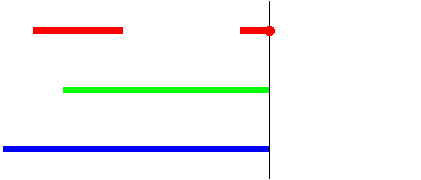
\includegraphics[width=.9\linewidth]{./figs/local-ind1.pdf}
\end{center}
\end{onlyenv}

\begin{onlyenv}<+>
\begin{center}
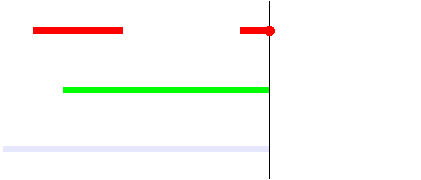
\includegraphics[width=.9\linewidth]{./figs/local-ind2.pdf}
\end{center}
\end{onlyenv}
\end{frame}

\begin{frame}[label={sec:orge546ce9}]{Local independence -- history}
Introduced by \cite{schweder1970composable} and elaborated and applied in \cite{aalen1987dynamic}
and \cite{aalen1980interaction}. \vfill \pause

Relation to graphical models considered by \cite{didelez2008graphical} and
\cite{mogensen2020markov}. \vfill \pause

\cite{aalen2016can} and \cite{aalen2012causality} discuss and give examples as to why local
independence might be better suited for modeling (causal) dependencies in a dynamical system. \vfill
\pause

\begin{quote} %% Quote
``We suggest that when people attempt to draw causal diagrams it is often most natural to think of
the nodes as processes and use local independence'' \citep[p.2300]{aalen2016can}.
\end{quote}
\end{frame}

\section{Advantages with LI}
\label{sec:orgd253c78}
\begin{frame}[label={sec:org9cd8fae}]{How might local independence be relevant in our setting?}
\pause
\begin{enumerate}
\item Model of temporal dependence \pause
\item An approach to mediation in a dynamical system \pause
\item ``Dynamic'' point of view
\end{enumerate}
\end{frame}
\begin{frame}[label={sec:org8dc5e16}]{1. Clustering disease patterns}
\begin{block}{Brunak Group}
\cite{jensen2014temporal} used Danish registries data to identify and cluster disease progressions.

\pause

\begin{center}
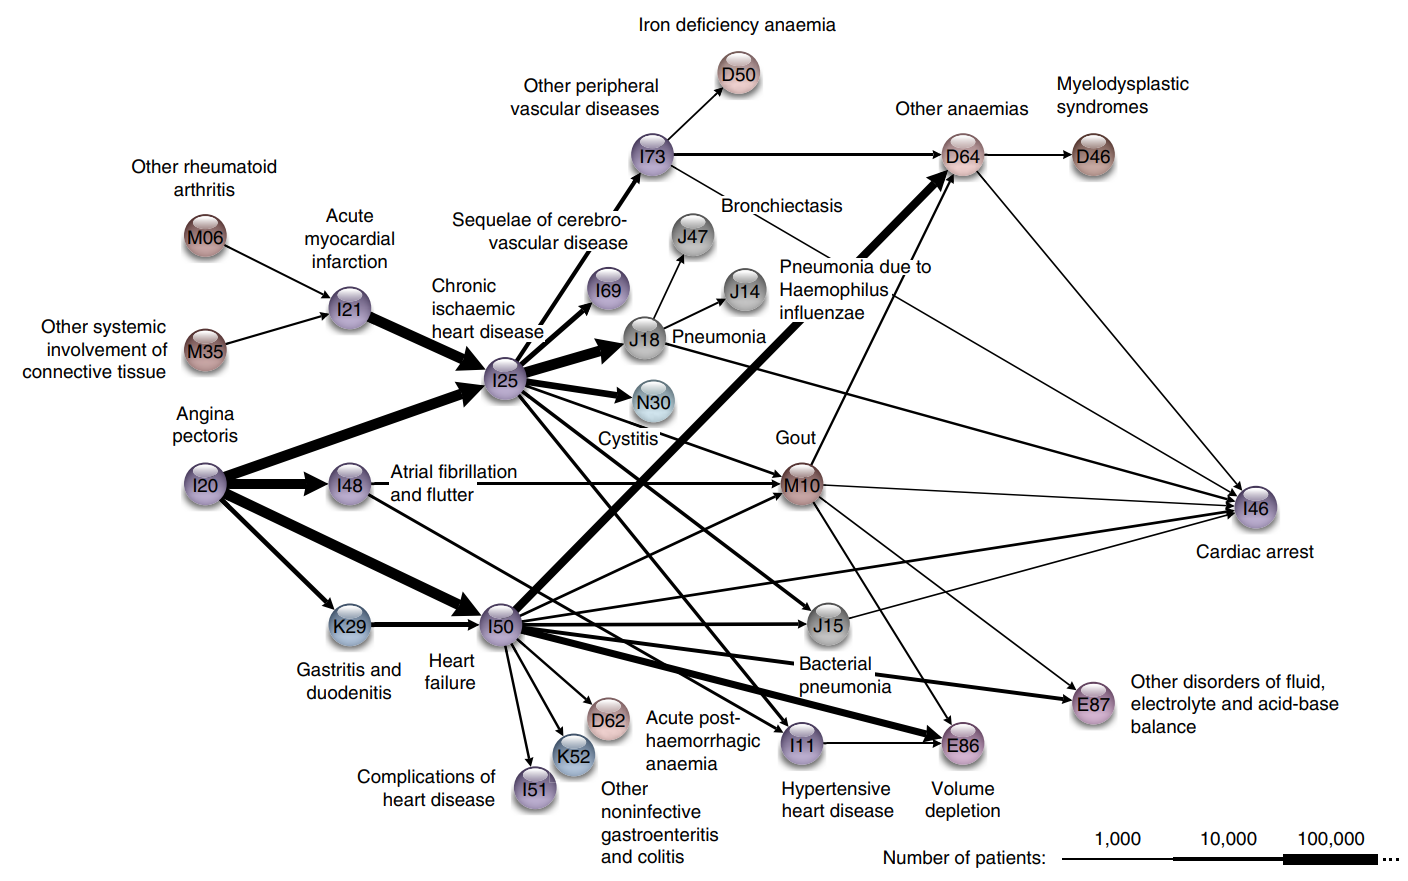
\includegraphics[width=.9\linewidth]{./figs/Brunak-disease-cluster.png}
\end{center}
\end{block}
\end{frame}

\begin{frame}[label={sec:orge7afa2a}]{1. Clustering disease patterns -- use local dependence?}
\begin{block}<+->{Brunak Group's approach to clustering}
\begin{itemize}
\item Matching every exposed patient to a non-exposed group with similar age and sex.
\item Test for association between diagnoses occurring within 4 years, and then test for ``temporal
direction''.
\item Various ad hoc choices.
\item Censoring and death not taken into account.
\item Interpretation unclear.
\end{itemize}
\end{block}

\begin{block}<+->{Try to use local dependence?}
\begin{itemize}
\item Better way to model ``temporal association''? Nicer interpretation?
\item Easier to handle stopped processes -- take death and censoring into account.
\item Perhaps fewer arbitrary choices.
\end{itemize}
\end{block}
\end{frame}

\begin{frame}[label={sec:org1cabb09}]{2. Mediation analysis in time}
Mediation analysis in time seems to be complicated. \pause

\begin{block}{Example:}
\begin{quote} %% counterfact survival quote
``To [\ldots{}] define the relevant direct and indirect effects in the survival context, we will have to
allow for hypothetical interventions on survival. [\ldots{}] The difficulty that otherwise arises is that
for those who do not survive the subsequent values of the mediator are always undefined. [\ldots{}] While
the mathematical development is precise, the interpretation of what such an intervention on survival
means is ambiguous.'' \citep[p.4154]{lin2017mediation}

\pause
\end{quote}
\end{block}
In addition, causal mechanisms can be ``smeared out'' or ``distorted'' by discretization
\citep{aalen2016can}.
\end{frame}

\begin{frame}[label={sec:org8730378}]{2. Mediation in time -- visualization}
\begin{onlyenv}<1>
\begin{center}
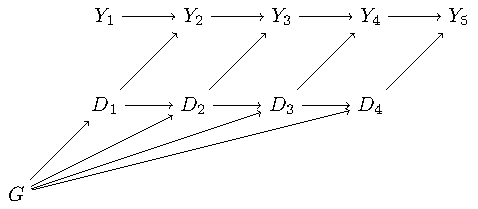
\includegraphics[width=.9\linewidth]{./figs/med-system.pdf}
\end{center}
\end{onlyenv}

\begin{onlyenv}<2>
\begin{center}
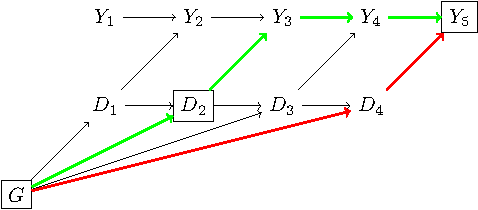
\includegraphics[width=.9\linewidth]{./figs/med-discrete-obs.pdf}
\end{center}
\end{onlyenv}

\begin{onlyenv}<3>
\begin{center}
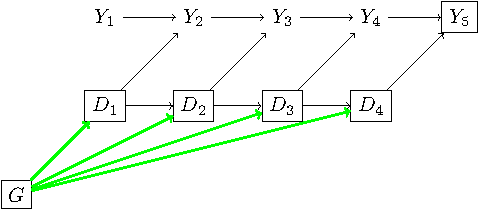
\includegraphics[width=.9\linewidth]{./figs/med-long1.pdf}
\end{center}
\end{onlyenv}

\begin{onlyenv}<4>
\begin{center}
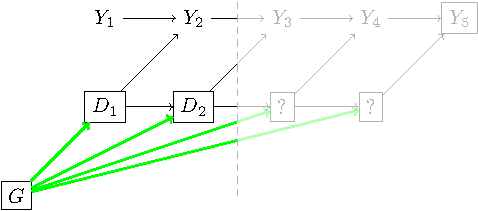
\includegraphics[width=.9\linewidth]{./figs/med-long2.pdf}
\end{center}
\end{onlyenv}

\begin{onlyenv}<5>
\begin{center}
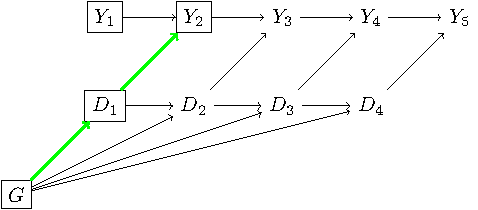
\includegraphics[width=.9\linewidth]{./figs/med-li1.pdf}
\end{center}
\end{onlyenv}

\begin{onlyenv}<6>
\begin{center}
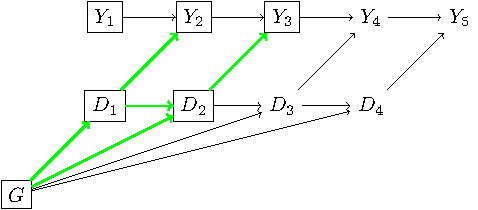
\includegraphics[width=.9\linewidth]{./figs/med-li2.pdf}
\end{center}
\end{onlyenv}

\begin{onlyenv}<7>
\begin{center}
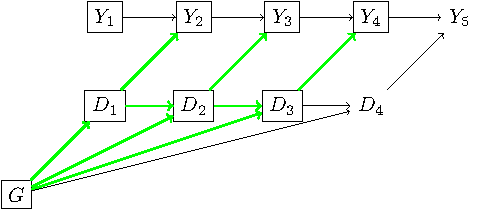
\includegraphics[width=.9\linewidth]{./figs/med-li3.pdf}
\end{center}
\end{onlyenv}

\begin{onlyenv}<8>
\begin{center}
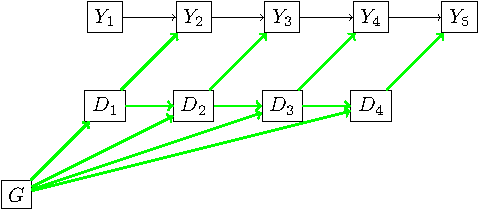
\includegraphics[width=.9\linewidth]{./figs/med-li4.pdf}
\end{center}
\end{onlyenv}
\end{frame}

\begin{frame}[label={sec:org3f5f883}]{2. Mediation analysis in time -- use local independence?}
\begin{quote} %% mechanistic mediation
``If a direct effect cannot reasonably be defined as a controlled or natural direct effect in the
counterfactual sense because the required hypothetical manipulation of the mediator is
inconceivable, then we can alternatively view these effects as being represented by flow in a
dynamic system, so that the direct effect corresponds to the flow not passing through the mediator.''
\citep{aalen2012causality}
\end{quote}
\end{frame}

\begin{frame}[label={sec:org3a576f1}]{3. Fixed time points (landmark analysis)}
\begin{block}<+->{Overcome the time problem by fixing time points}
Fix \(t_0\) and \(l >0\) and consider 
\begin{equation*}
  \P\left(Y(t_0 + l) = 1 \mid D(t_0), T > t_0 \right).
\end{equation*}

\begin{itemize}
\item Reasonable if \(t_0\) and \(t_0+l\) denote some meaningful time of intervention and follow-up time,
respectively.
\item Lose information about what happens between \(t_0\) and \(t_0 + l\).
\end{itemize}
\end{block}

\begin{block}<+->{Local independence}
\begin{itemize}
\item No need to fix time points.
\item Better to capture ``mechanistic workings''?
\end{itemize}
\end{block}
\end{frame}

\begin{frame}[label={sec:org415044e}]{Relevance of local independence (summary)}
\begin{enumerate}
\item Model of temporal dependence \(\rightarrow\) Better way to compare (stopped) processes. Use obtained
clusters as sub-diagnoses of HF.
\item An approach to mediation in a dynamical system \(\rightarrow\) Answer questions about causal pathways
for HF.
\item ``Dynamic'' point of view \(\rightarrow\) Allows a more ``exploratory'' approach.
\end{enumerate}
\end{frame}

\section{Challenges}
\label{sec:orga0bebe0}
\begin{frame}[label={sec:org4dd63a2}]{Major challenge}
\center Most likely it will \emph{not} hold that \(G \not \rightarrow Y \mid D\). Then what?

\vfill 

\begin{block}<2->{Effect estimation}
Could we construct a good measure for the ``strength'' of the dependence? Should this measure be
time-dependent? How should it be interpreted?
\end{block}

\begin{block}<3->{Time periods of dependence and independence?}
Would it be more informative to try and identify age spans during which dependence is present?
\end{block}
\end{frame}

\begin{frame}[label={sec:org60900a0}]{Other (major) challenges}
\begin{block}{Missing data}
Missing observations, censoring, selection bias, discretization.
\end{block}

\begin{block}{Interpretation}
Does the concept of local independence lead to models with a clear interpretation? Does it bring us
closer to causal interpretations -- and if so, in what sense?
\end{block}

\begin{block}{High-dimensional data}
Genes\ldots{} 
\end{block}
\end{frame}

\section{References}
\label{sec:orgad36848}
\begin{frame}[label={sec:org3c36440}]{References}
\tiny \bibliography{./bibliography.bib}
\end{frame}

\section{Final slide}
\label{sec:org0ca9517}
\begin{frame}[label={sec:org9761500}]{Questions / discussion}
\end{frame}
\section{Appendix}
\label{sec:orga08375f}
\appendix
\begin{frame}[label={sec:orge0838e7}]{Local independence -- mathematical definition}
$X(t)$ is a multivariate stochastic càdlàg process
\begin{equation*}
  X(t) = (X^1(t), X^2(t), \dots, X^k(t)), \quad t \in [0, T], 
\end{equation*}
on $[0,T]$. For any $C \subset V := \{1, \dots, k\}$ let $\mathcal{F}^C_t$ denote the completed and
right continuous version of $\sigma \{ X_s^c \, : \, s \leq t, c \in C\}$.

\vfill

For $\beta \in V, C \subset V$, let $\Lambda^{C, \beta}$ denote the compensator of
$\E[ X^{\beta}(t) \mid \mathcal{F}_t^C]$, i.e., $\Lambda^{C, \beta}$ is a
$\mathcal{F}_t^C$-predictable process and
\begin{equation*}
  \E[X^{\beta}(t) \mid \mathcal{F}_t^C] - \Lambda^{C, \beta}
\end{equation*}
is a martingale.

\vfill

Then for $A, B, C \subset V$, $X^B$ is said to be \textit{locally independent} of $X^A$ given $X^C$
if there exists an $\mathcal{F}_t^C$-predictable version of $\Lambda^{C \cup A, \beta}$ for all
$\beta \in B$. This is written as
\begin{equation*}
  A \not \rightarrow B \mid C.
\end{equation*}
\end{frame}
\end{document}